\documentclass[12pt,a4paper]{article}

\usepackage[provide=*,polish]{babel}
\usepackage[T1]{fontenc}
\usepackage[utf8]{inputenc}
\usepackage{lmodern}
\usepackage{geometry}
\usepackage{setspace}
\usepackage{amsmath}
\usepackage{amssymb}
\usepackage{booktabs}
\usepackage{graphicx}

\geometry{margin=2.2cm}
\setstretch{1.15}
\emergencystretch=2em
\graphicspath{{figures/}}

\begin{document}

\section{Liczba wyświetleń a Like Rate}

\textbf{Pytanie badawcze:} Jak zmieniał się Like Rate wraz ze wzrostem liczby wyświetleń filmu?

\begin{figure}[htbp]
    \centering
    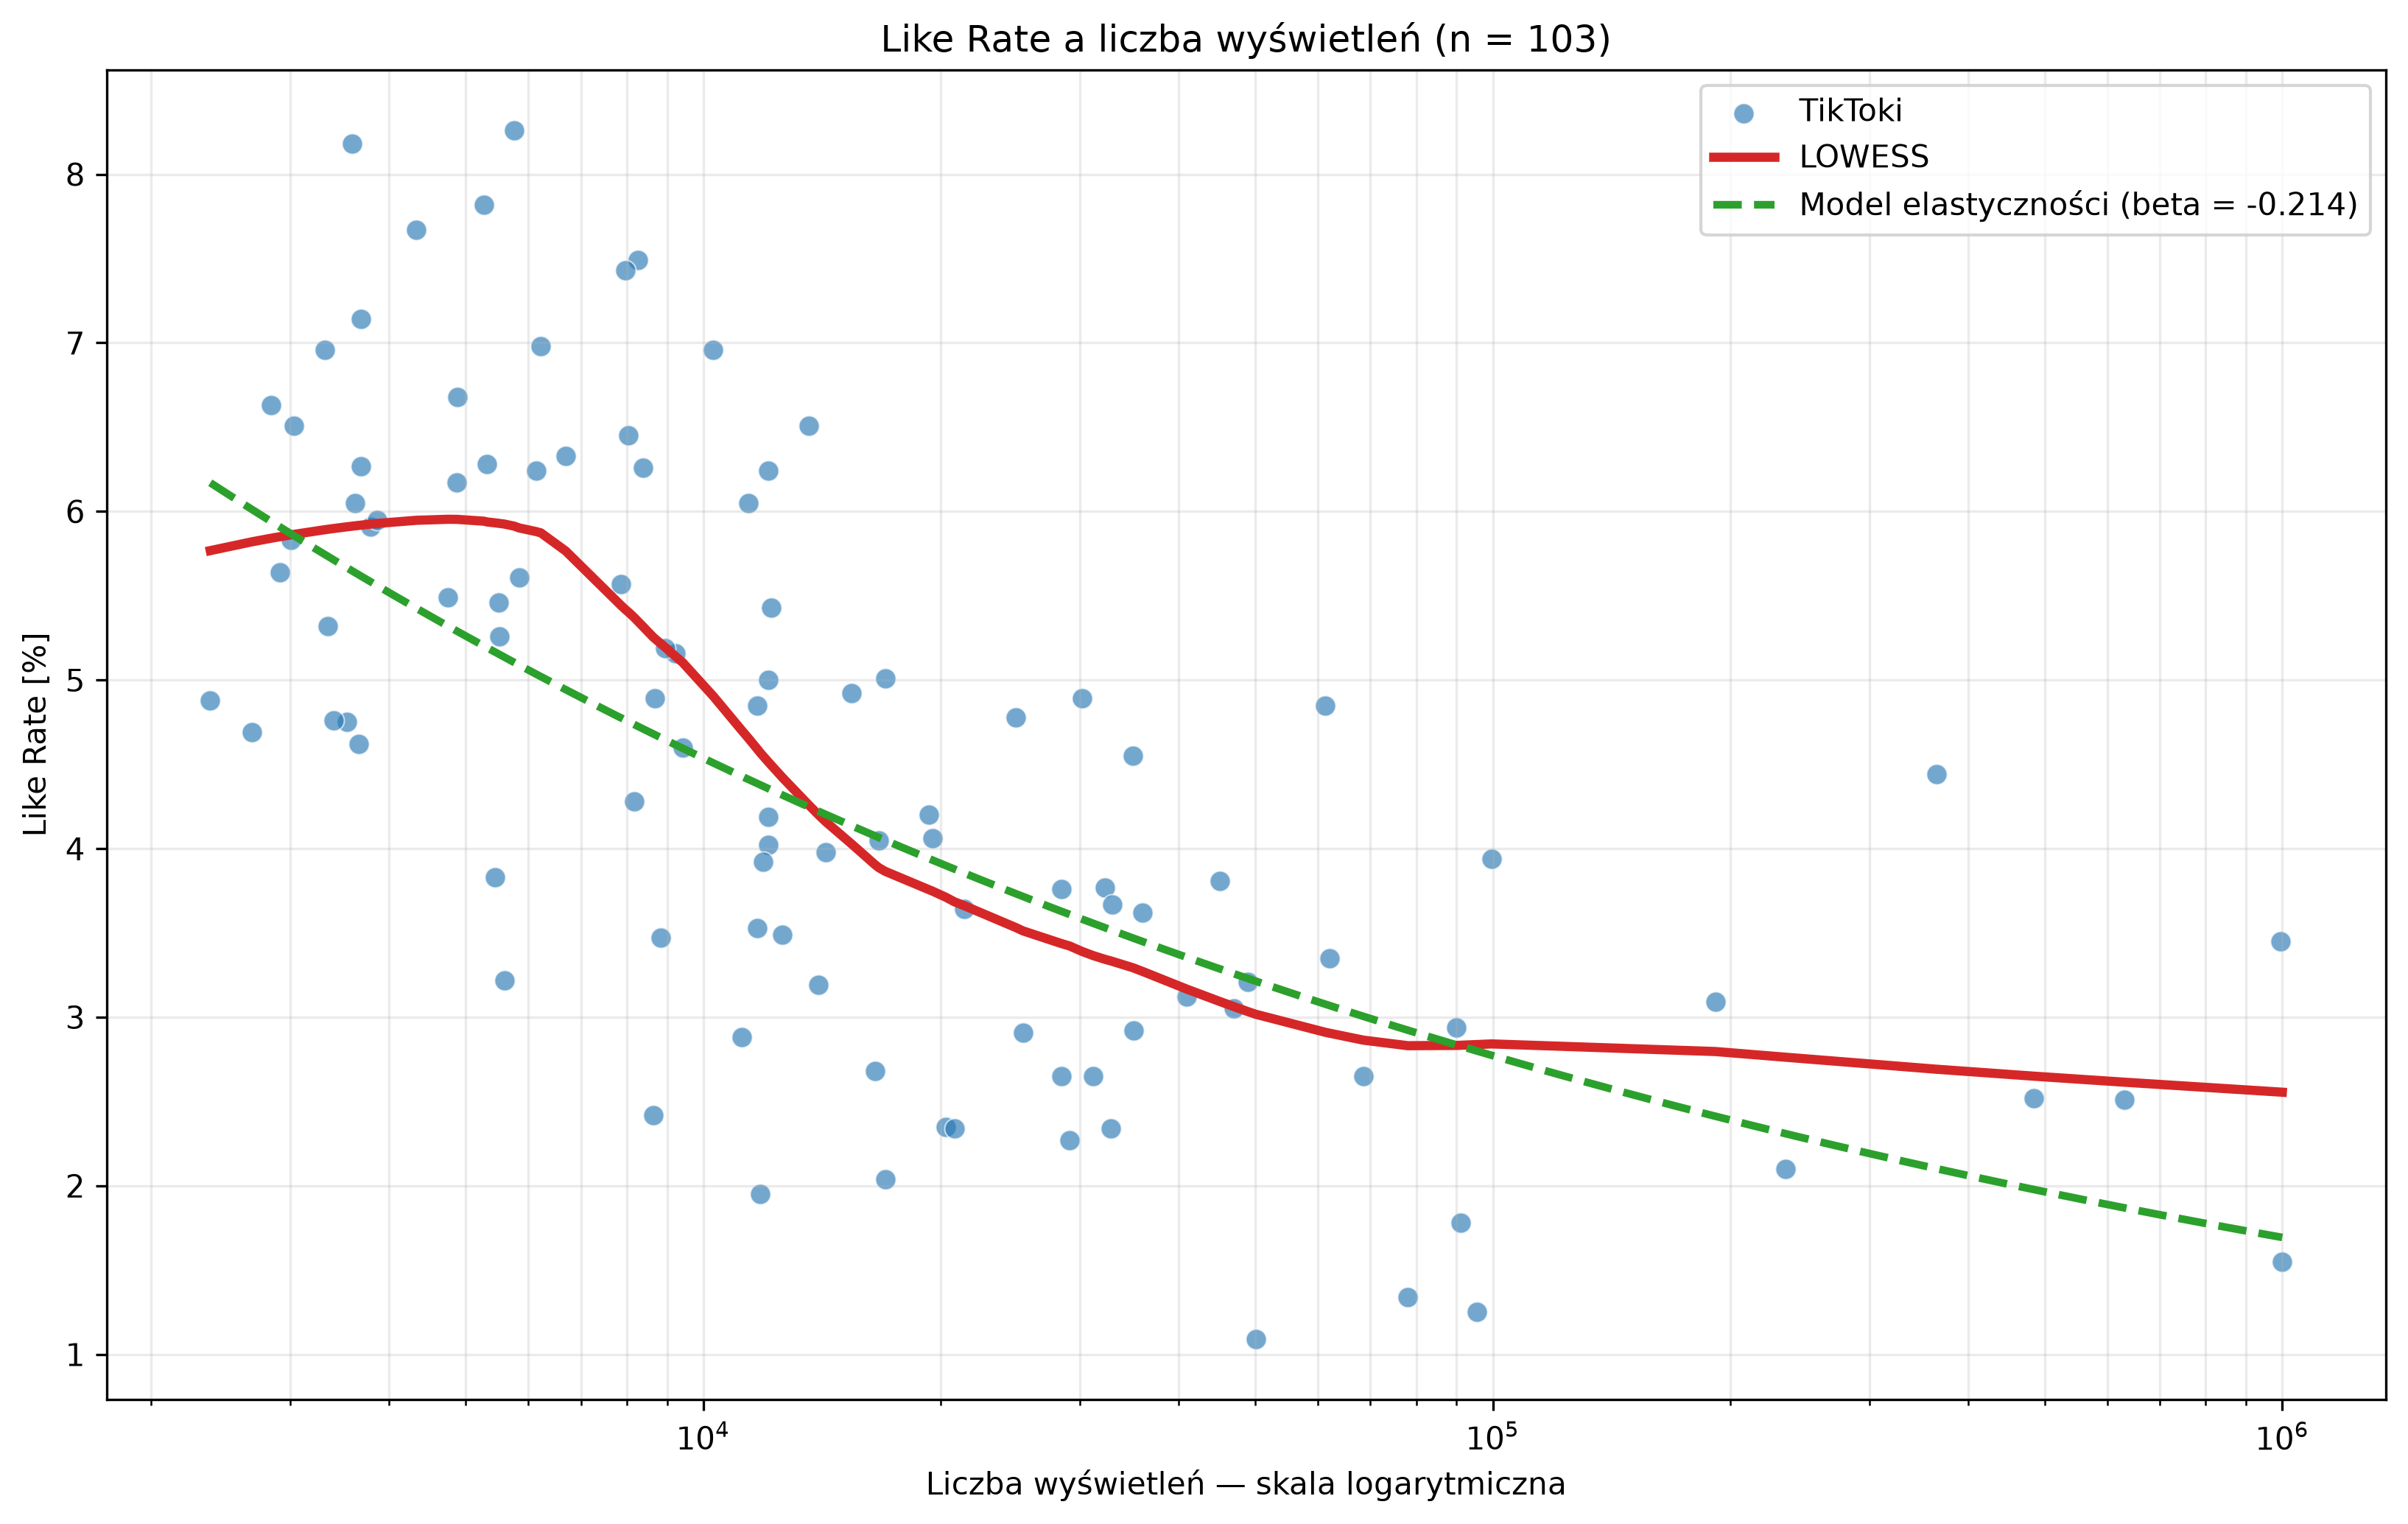
\includegraphics[width=\textwidth]{views_like_rate_lowess.png}
    \caption{Like Rate a liczba wyświetleń w pełnej próbie}
    \label{fig:pelna-proba}
\end{figure}

\subsection{Wykres punktowy i krzywa LOWESS}

Każda niebieska kropka na wykresie oznacza jeden film. Jej położenie na osi poziomej pokazuje liczbę wyświetleń, a położenie na osi pionowej --- Like Rate wyrażony w procentach. Oś liczby wyświetleń ma skalę logarytmiczną, ponieważ wartości mieszczą się w bardzo szerokim zakresie: od kilku tysięcy do około miliona wyświetleń.

W obliczeniach wykorzystano zmienne:

\[
x_i=\log_{10}(V_i),
\qquad
y_i=100L_i,
\qquad
L_i=\frac{\mathrm{Likes}_i}{V_i},
\]

gdzie $V_i$ oznacza liczbę wyświetleń $i$-tego filmu, a $L_i$ jego Like Rate zapisany jako ułamek.

Aby dokładnie odtworzyć wyniki otrzymane wcześniej z widoku bazy danych, przed obliczeniami Like Rate zaokrąglono do czterech miejsc po przecinku. Odpowiada to dokładności $0{,}01$ punktu procentowego.

Czerwona linia została wyznaczona metodą LOWESS. Nie zakłada ona z góry, że zależność ma być liniowa, kwadratowa albo wykładnicza. Zamiast dopasowywać jedną funkcję do całej próby, LOWESS dopasowuje wiele lokalnych prostych. Dla kolejnych miejsc na osi $X$ wybiera najbliższe obserwacje, nadaje większą wagę punktom położonym bliżej, dopasowuje do nich prostą i zapisuje jej przewidywaną wartość. Połączenie tych lokalnych przewidywań tworzy czerwoną krzywą.

\subsubsection*{Jak działa LOWESS w tej analizie}

\begin{enumerate}
    \item \textbf{Wybór badanego miejsca}

    Wybieramy punkt $x_0$, dla którego chcemy oszacować wygładzoną wartość Like Rate.

    \item \textbf{Obliczenie odległości}

    Dla każdej obserwacji obliczamy odległość od badanego miejsca:

    \[
    d_i=\lvert x_i-x_0\rvert.
    \]

    \item \textbf{Wybór najbliższych obserwacji}

    Parametr \texttt{frac} ustawiono na $0{,}4854$. Oznacza to, że do każdego lokalnego dopasowania wykorzystywane jest około

    \[
    0{,}4854\cdot 103\approx 50
    \]

    najbliższych filmów. Parametr \texttt{frac} steruje stopniem wygładzenia: mniejsza wartość daje bardziej elastyczną krzywą, a większa --- gładszą.

    \item \textbf{Nadanie wag zależnych od odległości}

    Niech $h$ oznacza największą odległość od $x_0$ wśród obserwacji wybranych do lokalnego dopasowania. Definiujemy:

    \[
    u_i=\frac{d_i}{h}.
    \]

    Waga odległościowa ma postać funkcji trójsześciennej:

    \[
    w_i^{(d)}=
    \begin{cases}
        \left(1-u_i^3\right)^3, & 0\leq u_i<1,\\
        0, & u_i\geq 1.
    \end{cases}
    \]

    Im bliżej $x_i$ znajduje się punktu $x_0$, tym większą otrzymuje wagę. Punkty leżące poza lokalnym sąsiedztwem mają wagę równą zeru.

    \item \textbf{Dopasowanie lokalnej prostej}

    W wybranym sąsiedztwie dopasowujemy ważoną prostą:

    \[
    \widehat{y}=a+bx.
    \]

    Oznaczmy przez $\omega_i$ całkowitą wagę obserwacji. W pierwszym przejściu jest to waga odległościowa $w_i^{(d)}$. Średnie ważone wynoszą:

    \[
    \overline{x}_{\omega}
    =
    \frac{\sum_i \omega_i x_i}{\sum_i \omega_i},
    \qquad
    \overline{y}_{\omega}
    =
    \frac{\sum_i \omega_i y_i}{\sum_i \omega_i}.
    \]

    Współczynnik nachylenia lokalnej prostej jest równy:

    \[
    b=
    \frac{
        \sum_i \omega_i
        (x_i-\overline{x}_{\omega})
        (y_i-\overline{y}_{\omega})
    }{
        \sum_i \omega_i
        (x_i-\overline{x}_{\omega})^2
    },
    \]

    natomiast wyraz wolny:

    \[
    a=\overline{y}_{\omega}-b\overline{x}_{\omega}.
    \]

    Wartość krzywej LOWESS w badanym miejscu wynosi więc:

    \[
    \widehat{y}(x_0)=a+bx_0.
    \]

    \item \textbf{Ograniczenie wpływu obserwacji odstających}

    W kodzie ustawiono \texttt{it=3}, dlatego po początkowym dopasowaniu wykonywane są trzy dodatkowe ważenia na podstawie reszt. Filmy o dużych resztach, czyli położone daleko od lokalnej prostej, otrzymują mniejszą wagę. Obserwacje z resztą większą niż sześciokrotność mediany bezwzględnych reszt mogą otrzymać wagę równą zeru. Dzięki temu pojedynczy nietypowy film ma mniejszy wpływ na przebieg czerwonej linii.
\end{enumerate}

Cała procedura jest powtarzana dla kolejnych wartości $x_0$. Czerwona linia nie łączy więc bezpośrednio obserwowanych punktów, lecz przedstawia ciąg lokalnych oszacowań Like Rate.

\subsubsection*{Odczyt krzywej}

\begin{itemize}
    \item przy kilku tysiącach wyświetleń wygładzony Like Rate wynosi około $5{,}7$--$6{,}0\%$
    \item w zakresie od około $7$--$10$ tys. do $50$--$70$ tys. wyświetleń widoczny jest wyraźny spadek Like Rate
    \item powyżej około $70$--$100$ tys. wyświetleń krzywa wypłaszcza się w pobliżu $2{,}6$--$2{,}9\%$
\end{itemize}

LOWESS służy tutaj do opisania kształtu zależności. Sam wykres nie pokazuje, że wzrost liczby wyświetleń powoduje spadek Like Rate.

\subsection{Korelacja rang Spearmana}

Korelację Spearmana zastosowano zamiast korelacji Pearsona, ponieważ liczba wyświetleń jest silnie asymetryczna, część filmów osiąga nietypowo duże zasięgi, a zależność widoczna na wykresie nie jest liniowa. Spearman mierzy siłę zależności monotonicznej na podstawie rang, a nie bezpośrednio na podstawie surowych wartości.

Niech $R_i$ oznacza rangę liczby wyświetleń, a $S_i$ rangę Like Rate. Współczynnik Spearmana jest korelacją Pearsona między tymi rangami:

\[
\rho_S=
\frac{
    \sum_{i=1}^{n}(R_i-\overline{R})(S_i-\overline{S})
}{
    \sqrt{\sum_{i=1}^{n}(R_i-\overline{R})^2}
    \sqrt{\sum_{i=1}^{n}(S_i-\overline{S})^2}
}.
\]

W pełnej próbie otrzymano:

\[
\rho_S=-0{,}7212,
\qquad
95\%\ \mathrm{CI}=[-0{,}7863;\,-0{,}6333],
\]

\[
p=8{,}5878\cdot 10^{-18},
\qquad
n=103.
\]

Wartość $\rho_S=-0{,}7212$ oznacza silną ujemną zależność rangową: filmy z większą liczbą wyświetleń miały zazwyczaj niższy Like Rate. Interpretujemy wartość bezwzględną współczynnika, czyli $\lvert\rho_S\rvert=0{,}7212$, natomiast znak minus określa kierunek zależności.

Przedział ufności wyznaczono metodą bootstrapu. Dziesięć tysięcy razy losowano ze zwracaniem całe pary \emph{liczba wyświetleń--Like Rate}, a następnie dla każdej wylosowanej próby ponownie obliczano $\rho_S$. Granice przedziału są percentylami $2{,}5\%$ i $97{,}5\%$ otrzymanych współczynników.

Cały przedział $[-0{,}7863;\,-0{,}6333]$ znajduje się poniżej zera, co wspiera wniosek o ujemnym kierunku zależności. Bardzo mała wartość $p$ oznacza, że przy hipotezie zerowej o braku monotonicznej zależności uzyskanie współczynnika co najmniej tak odległego od zera byłoby bardzo mało prawdopodobne. Wynik jest istotny statystycznie, ale nie dowodzi zależności przyczynowej.

\subsection{Model elastyczności}

Do ilościowego opisania zależności zastosowano model log--log:

\[
\ln(L_i)=\alpha+\beta\ln(V_i)+\varepsilon_i,
\]

gdzie $L_i$ oznacza Like Rate, a $V_i$ liczbę wyświetleń. W pełnej próbie oszacowano:

\[
\widehat{\ln(L_i)}
=
-1{,}1225-0{,}2139\ln(V_i).
\]

Otrzymano:

\[
\widehat{\beta}=-0{,}2139,
\qquad
95\%\ \mathrm{CI}=[-0{,}2750;\,-0{,}1529],
\]

\[
p=3{,}6122\cdot 10^{-10},
\qquad
R^2=0{,}4300,
\qquad
n=103.
\]

W modelu log--log współczynnik $\beta$ jest elastycznością. Wzrost liczby wyświetleń o $1\%$ wiązał się przeciętnie ze spadkiem Like Rate o około $0{,}214\%$. Jest to zmiana względna Like Rate, a nie spadek o $0{,}214$ punktu procentowego.

Dokładną względną zmianę Like Rate przy $k$-krotnym wzroście liczby wyświetleń obliczamy ze wzoru:

\[
100\left(k^{\widehat{\beta}}-1\right)\%.
\]

Dla pełnej próby wzrost liczby wyświetleń o $10\%$ odpowiadał przeciętnemu spadkowi Like Rate o około $2{,}02\%$, a podwojenie liczby wyświetleń --- spadkowi o około $13{,}79\%$.

Cały przedział ufności dla $\beta$ znajduje się poniżej zera. Model z jedną zmienną objaśnia około $43{,}0\%$ zróżnicowania logarytmu Like Rate. Zastosowano odporne błędy standardowe HC3. Wyrazu wolnego nie interpretujemy praktycznie, ponieważ odpowiada on filmowi z jednym wyświetleniem, czyli sytuacji znajdującej się poza użytecznym zakresem danych.

\section{Analiza odporności po wyłączeniu TOP 7}

\begin{figure}[htbp]
    \centering
    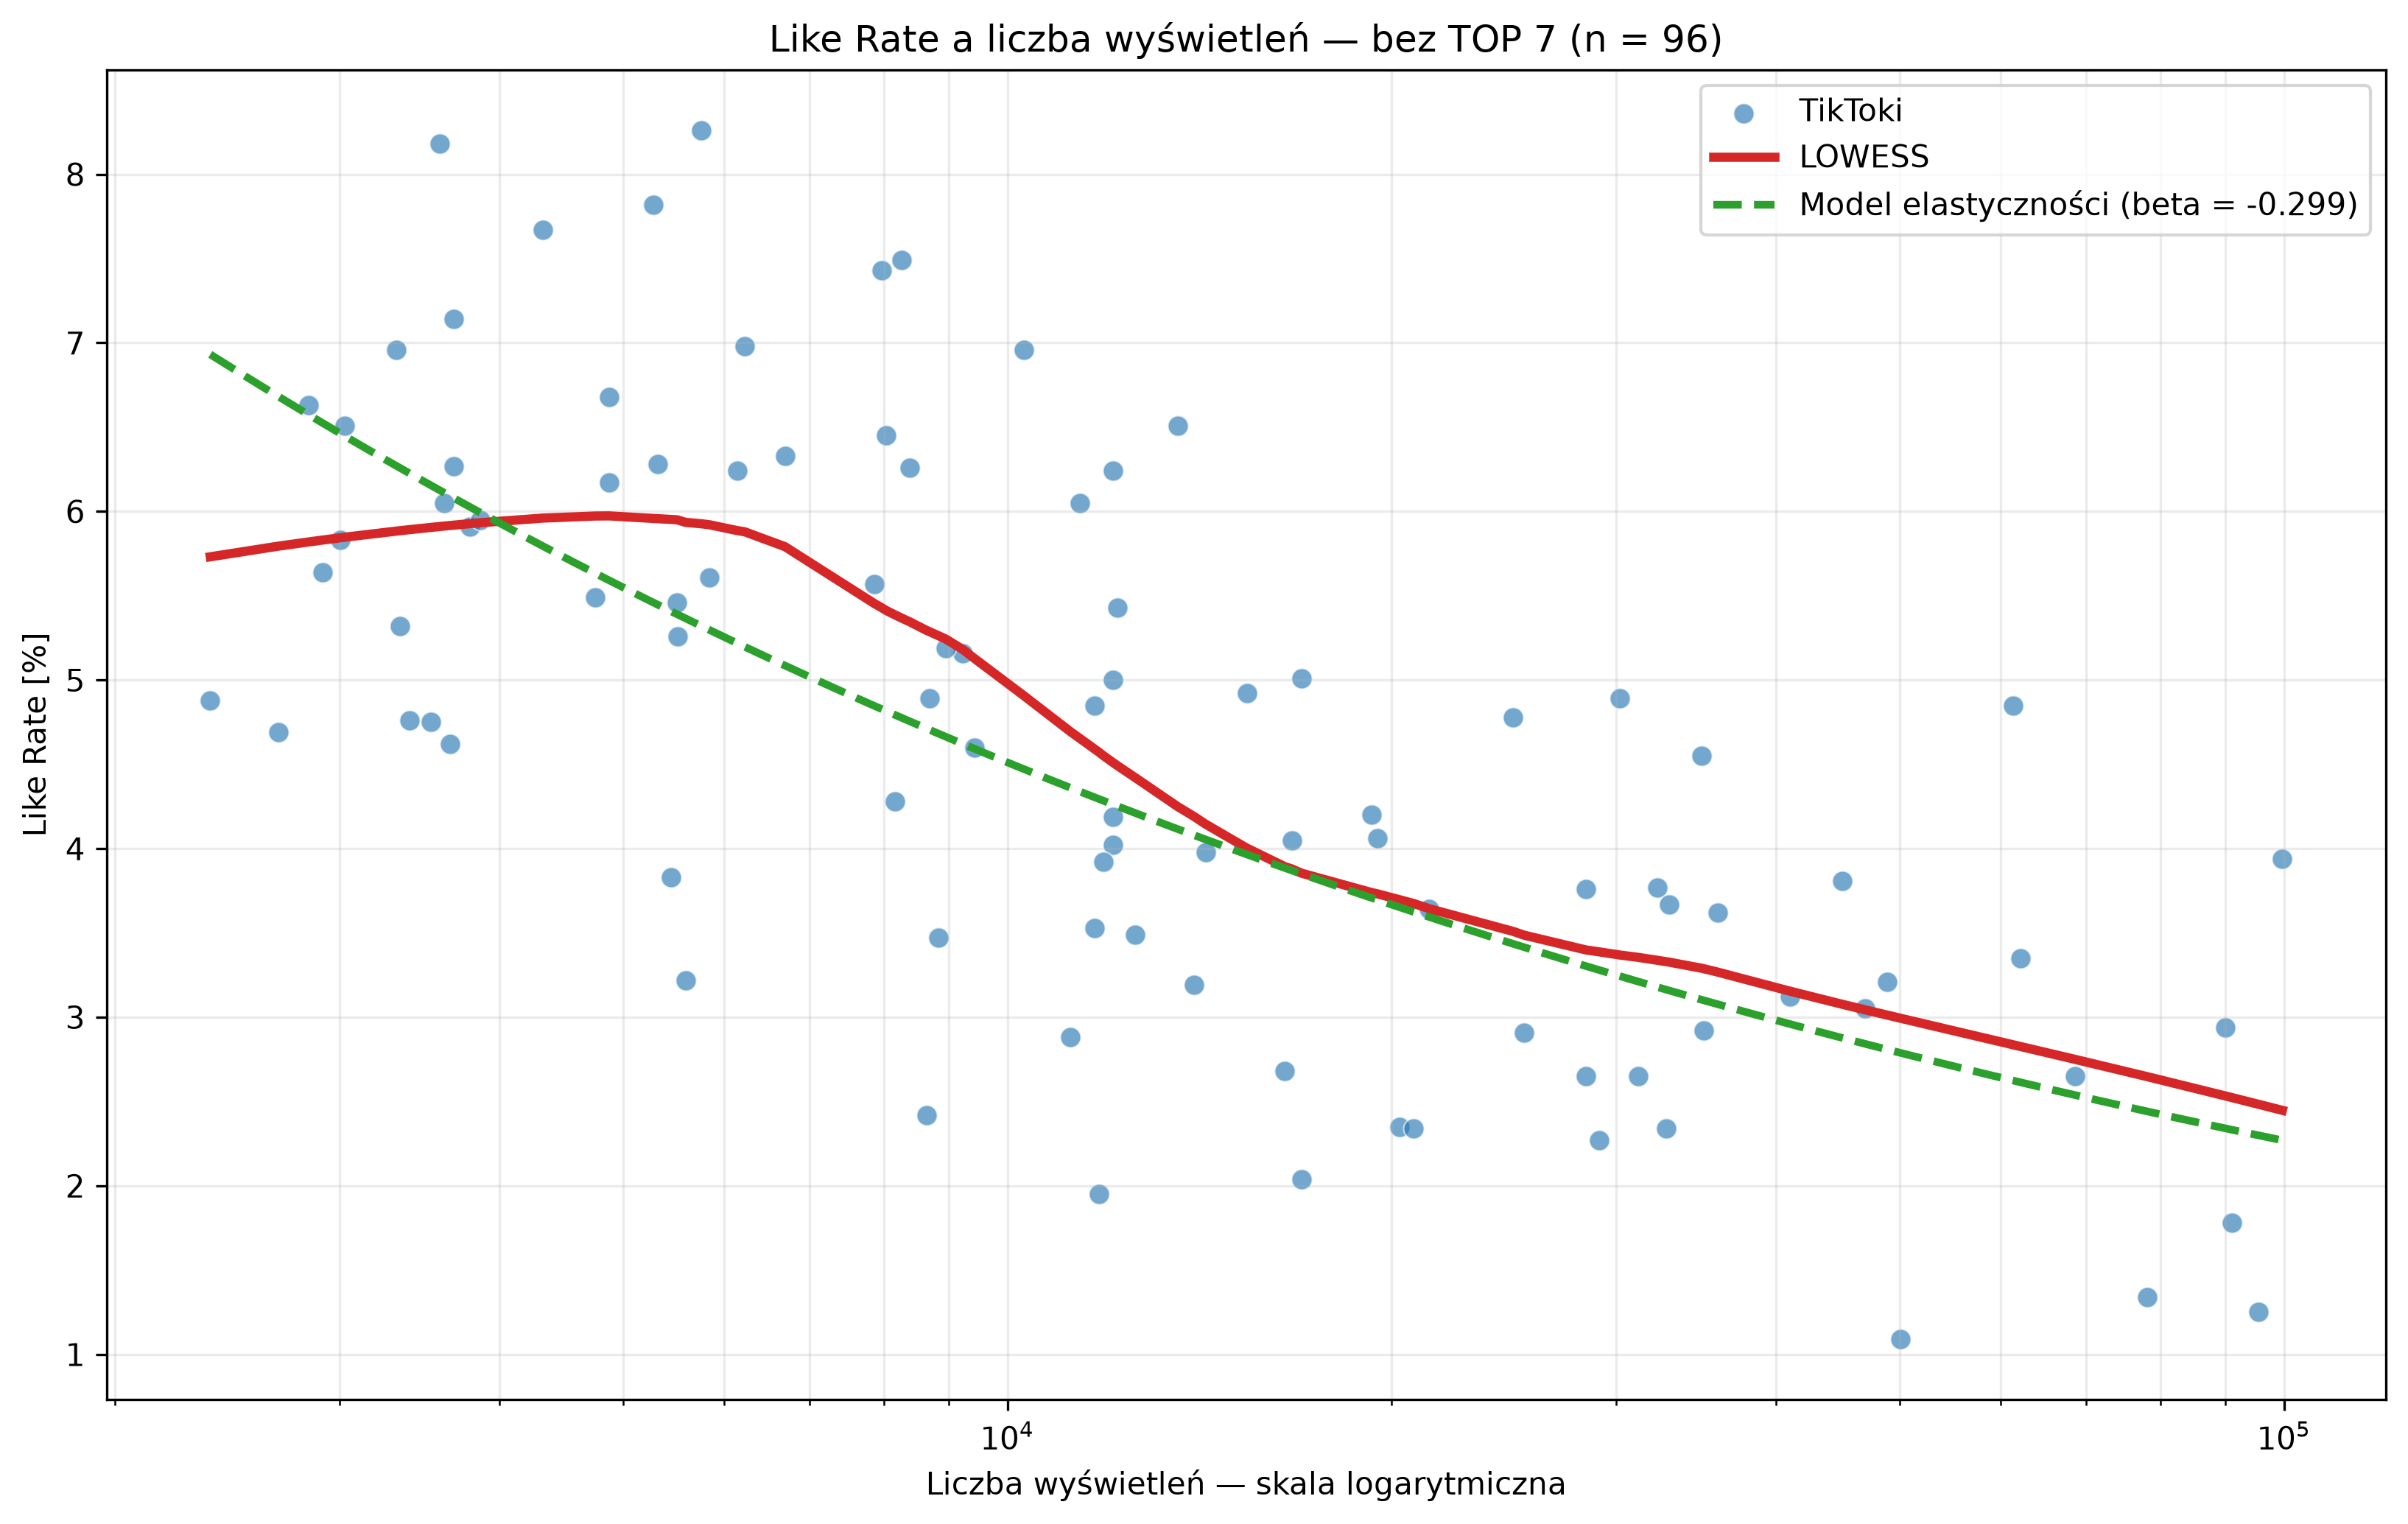
\includegraphics[width=\textwidth]{views_like_rate_without_top7.png}
    \caption{Like Rate a liczba wyświetleń po wyłączeniu siedmiu filmów o największym zasięgu}
    \label{fig:bez-top7}
\end{figure}

Siedem filmów o największej liczbie wyświetleń wyłączono wyłącznie w analizie odporności. Nie oznacza to uznania ich za błędne obserwacje. Celem było sprawdzenie, czy wynik pełnej próby nie jest w całości napędzany przez filmy o największym zasięgu. Po ich wyłączeniu pozostało:

\[
n=96.
\]

W zakresie wspólnym dla obu wykresów kształt krzywej LOWESS pozostał podobny. Nadal widoczny jest niewielki początkowy wzrost, następnie silny spadek i późniejsze łagodzenie spadku. Oznacza to, że ujemna zależność nie wynika wyłącznie z siedmiu filmów o największej liczbie wyświetleń. Jednocześnie to właśnie te filmy tworzą prawy, viralowy fragment pełnego wykresu, na którym krzywa wyraźnie się wypłaszcza.

\subsection{Korelacja rang Spearmana}

\noindent
Po wyłączeniu TOP 7 otrzymano:

\[
\rho_S=-0{,}6993,
\qquad
95\%\ \mathrm{CI}=[-0{,}7744;\,-0{,}5996],
\]

\[
p=2{,}2811\cdot 10^{-15},
\qquad
n=96.
\]

Zmiana oszacowania wyniosła:

\[
-0{,}6993-(-0{,}7212)=0{,}0219.
\]

Współczynnik stał się więc nieznacznie mniej ujemny, ale zależność nadal jest silna. Przedziały ufności obu oszacowań w dużym stopniu się pokrywają. Samo nakładanie się przedziałów nie jest jednak formalnym testem różnicy między korelacjami, dlatego na tej podstawie nie stwierdzamy ani istotności, ani nieistotności zmiany.

\subsection{Model elastyczności}

\noindent
Po wyłączeniu TOP 7 oszacowano:

\[
\widehat{\ln(L_i)}
=
-0{,}3472-0{,}2987\ln(V_i).
\]

Otrzymano:

\[
\widehat{\beta}=-0{,}2987,
\qquad
95\%\ \mathrm{CI}=[-0{,}3731;\,-0{,}2244],
\]

\[
p=3{,}5728\cdot 10^{-12},
\qquad
R^2=0{,}4750,
\qquad
n=96.
\]

Wzrost liczby wyświetleń o $1\%$ wiązał się przeciętnie ze spadkiem Like Rate o około $0{,}299\%$. Wzrost liczby wyświetleń o $10\%$ odpowiadał spadkowi Like Rate o około $2{,}81\%$, a podwojenie liczby wyświetleń --- spadkowi o około $18{,}70\%$.

Dla pełnej próby otrzymano $\widehat{\beta}_{\text{pełna}}=-0{,}2139$, natomiast po wyłączeniu TOP 7:

\[
\widehat{\beta}_{\mathrm{bez\ TOP\ 7}}=-0{,}2987.
\]

Różnica oszacowań wyniosła:

\[
-0{,}2987-(-0{,}2139)=-0{,}0848.
\]

Oszacowana zależność stała się bardziej ujemna. Jest to zgodne z krzywą LOWESS: w typowym zakresie zasięgów Like Rate wyraźnie spadał, natomiast w prawym, viralowym fragmencie pełnej próby spadek ulegał wypłaszczeniu. Nie oznacza to jednak, że różnica między współczynnikami $-0{,}2139$ i $-0{,}2987$ jest statystycznie istotna. Do takiego wniosku potrzebny byłby osobny test.

Model bez TOP 7 wyjaśnia około $47{,}5\%$ zróżnicowania logarytmu Like Rate.

\subsection{Porównanie wyników}

\begin{center}
\begin{tabular}{lcc}
\toprule
Miara & Pełna próba & Bez TOP 7 \\
\midrule
Liczba filmów $n$ & $103$ & $96$ \\
Korelacja Spearmana $\rho_S$ & $-0{,}7212$ & $-0{,}6993$ \\
Elastyczność $\widehat{\beta}$ & $-0{,}2139$ & $-0{,}2987$ \\
$R^2$ modelu log--log & $0{,}4300$ & $0{,}4750$ \\
\bottomrule
\end{tabular}
\end{center}

Analiza odporności prowadzi do dwóch wniosków. Po pierwsze, ujemna zależność rangowa pozostaje silna po wyłączeniu największych filmów. Po drugie, oszacowana elastyczność staje się bardziej ujemna, ponieważ usunięto fragment danych, w którym spadek Like Rate wcześniej się wypłaszczał. W żadnym z modeli nie należy interpretować tej zależności jako dowodu, że większa liczba wyświetleń sama w sobie powoduje niższy Like Rate.

\end{document}
